\documentclass[handout]{beamer}
%\documentclass{beamer}

% \usetheme{boxes} % see http://www.deic.uab.es/~iblanes/beamer_gallery/ for lots of examples
\usetheme{metropolis}
\usecolortheme{rose}
% \useinnertheme{circles}
% \useoutertheme{split}
% \setbeamertemplate{blocks}[rounded][shadow=true]

\setbeamertemplate{navigation symbols}{} % remove navigation symbols
\setbeamertemplate{footline}{} % remove title, too long

% %next set colors - not needed
% \setbeamercolor{title}{fg=black!70!black}
% \setbeamercolor{frametitle}{fg=blue!70!black}
% \setbeamercolor{framesubtitle}{fg=green!30!black}
% \setbeamercolor{author}{fg=red!70!black}
% \setbeamercolor{institute}{fg=green!30!black}
% \setbeamercolor{date}{fg=blue!50!black}

% \usepackage[T1]{fontenc}        % kodiranje znakov v .pdf
% \usepackage[utf8]{inputenc}     % kodiranje znakov v .tex
% \usepackage[slovene]{babel}     % nastavimo slovenščino
% \usepackage{stmaryrd}

\usepackage{fontspec}
\usepackage{unicode-math}
\usepackage{enumerate}

\usepackage{graphicx}

% \setmainfont{Latin Modern Sans}
\setmathfont{Latin Modern Math}
\setmathfont{Asana Math}[range={scr}]
\setmathfont{STIX Two Math-Regular}[range={bb}]
\setmathfont{Asana Math}[range={8709}]  % U+2205, emptyset
\setmathfont{Asana Math}[range={10631, 10632}]  % U+2987, U+2988, bb parenthesis

\usepackage{ulem}
\renewcommand{\ULdepth}{1.8pt}
\newcommand{\ul}[1]{\uline{#1}}

% \newtheorem{theorem}{Izrek}
% \newtheorem{statement}{Trditev}
% \newtheorem{lemma}{Lema}
% \newtheorem*{corrolary}{Posledica}

% \theoremstyle{definition}
% \newtheorem{definition}{Definicija}

% \newtheorem*{example}{Primer}
% \newtheorem*{example*}{Primer}
% \newtheorem*{examples}{Primeri}

% \theoremstyle{remark}
% \newtheorem*{remark}{Opomba}

% \beamertemplatetransparentcovereddynamic

\title{Choice axioms and real numbers}
\author{Luna Strah}
\institute{University of Ljubljana}
\date{19.~9.~2024}

% \newcommand{\vphi}{\phi}
\renewcommand{\phi}{\varphi}
\newcommand{\eps}{\varepsilon}
\renewcommand{\hat}{\widehat}
\renewcommand{\tilde}{\widetilde}
% \newcommand{\oldbar}{\bar}
% \renewcommand{\bar}{\overline}
\newcommand{\subs}{\subseteq}
\newcommand{\nin}{\not\in}

\newcommand{\p}[1]{\left( {#1} \right)}
\renewcommand{\b}[1]{\left[ {#1} \right]}
\newcommand{\set}[2]{\left\{ #1 \mid #2 \right\}}
\newcommand{\newfrac}[2]{{}^{#1}\!/_{\!#2}}
\newcommand{\smallfrac}[2]{{\textstyle\frac{#1}{#2}}}
\newcommand{\im}[1]{\mathrm{im}{\p{#1}}}
\newcommand{\mb}[1]{\mathbb{#1}}
\newcommand{\mf}[1]{\mathfrak{#1}}
\newcommand{\mc}[1]{\mathcal{#1}}
\newcommand{\id}{\mathrm{id}}

\def\bN{\mb{N}}
\def\bR{\mb{R}}
\def\alpo{\mathrm{ALPO}}
\def\ac#1{\mathrm{AC}{\left(#1\right)}}
\def\acn#1{\ac{\bN, #1}}
\def\sh#1{\mathrm{Sh}{\left(#1\right)}}
\def\subq{\subseteq}
\def\forces{\Vdash}
\def\phi{\varphi}
\def\Rd{\bR_d}
\def\Rc{\bR_c}


\newcommand{\sem}[1]{⟦ #1 ⟧}
% \newcommand{\brsem}[1]{⟬ #1 ⟭}
% \newcommand{\brsem}[1]{⦅ #1 ⦆}
\newcommand{\brsem}[1]{⦇ #1 ⦈}

\newcommand{\airquotes}[1]{"#1"}


% \setbeameroption{hide notes} % Only slides
% \setbeameroption{show only notes} % Only notes
% \setbeameroption{show notes} % Both
\setbeameroption{show notes on second screen=right} % Both


\begin{document}
%%%%%
\frame{\titlepage
\note{
    I plan to take you on the journey I took to discovering a cute minor result.

    There are various ways to define the real numbers, in particular we're interested in the Dedekind and Cauchy reals.

    Classically, these give the same objects, in particular LEM or CC are enough.
}
}
%%%%%

\begin{frame}
    \frametitle{Countable choice implies the Dedekind and Cauchy reals are the same}

    \begin{proof}
        Take Dedekind cut \(\p{L_x,U_x}\).
        We construct a sequence of rational interval approximations \(\p{p_n, q_n}\) as follows:
        Take arbitrary \(p_0 \in L_x\) and \(q_0 \in U_x\). Then at step \(n+1\) define
        \begin{align*}
            a = \frac{2p_n + q_n}{3}\qquad b = \frac{p_n + 2q_n}{3}
        \end{align*}
        Now define \(\p{p_{n+1}, q_{n+1}} \coloneq \begin{cases} \p{a, q_n} &; a \in L_x\\\p{p_n, b} &; b \in U_x\end{cases}\).
    \end{proof}

    \begin{figure}
        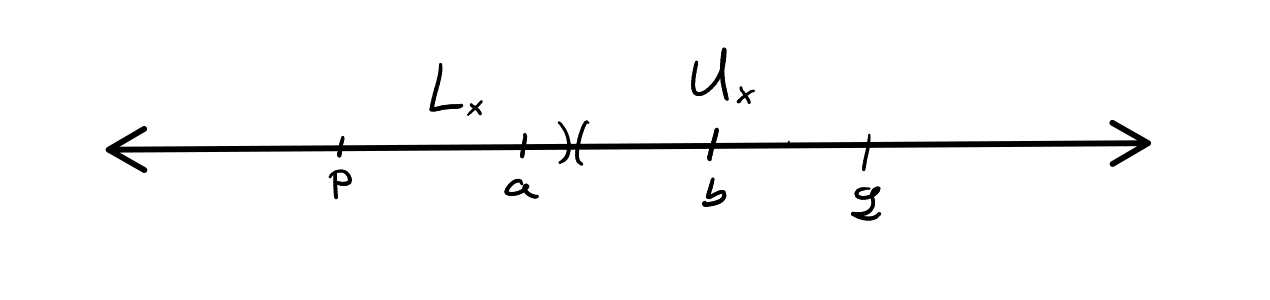
\includegraphics[width=0.7\textwidth]{real-line-export-2.png}
    \end{figure}

    \note{
        The proof is simple once you see it. We represent Dedekind reals by two-sided Dedekind cuts and the Cauchy reals by sequences of rational interval approximations.

        Take arbitrary points in each of the cuts, then inductively at step \(n\) look at the thirds and choose an interval that contains the real \(x\).

        So, this uses countable choice, and in particular, CC for binary sets. Call it \(\acn2\).

        %This proof also works with LEM, however LEM also implies \(\acn2\), so we only consider that.

        Now Andrej Bauer has been asking people for more than 10 years whether we can recover some sort of choice principle by assuming that Dedekind reals are Cauchy. I answer this in the negative.
    }
\end{frame}

\begin{frame}
    \frametitle{The reals, really}

    For sheaf toposes over topological spaces \(\Rd = \mc{C}{\p{-, \bR}}\).

    Further, if the space is locally connected, \(\Rc = \uline{\bR}\).

    \pause
    So the objects \(\Rd\) and \(\Rc\) are the same when every continuous function from a subset of \(X\) to the reals is locally constant.

    \note{
        Now in sheaf topoi over spaces we know what each of the constructions of reals look like, externally as sheaves.

        The Dedekind reals are simply the functions from open subsets to the reals,
        while the Cauchy reals are the locally constant such functions (for locally connected spaces).

        So, in the topos \(\Rd = \Rc\) when all local functions to reals are locally constant.
    }
\end{frame}

\begin{frame}
    \frametitle{\(\acn2\) in \(\sh{X}\)}

    Call a P-space a topological space in which any countable intersection of open sets is open.

    Then if a space is \(T_1\) and in the sheaf topos over it \(\acn2\) holds it must be a P-space.
    % Then in the sheaf topos over any P-space \(\acn2\) holds.

    % \pause
    % Furthermore, if the space is \(T_1\) the converse holds.

    % (\(X \not\forces \acn2\) implies \(X\) not a P-space or \(X\) not \(T_1\))

    \pause
    Thus, we want a space such that
    \begin{enumerate}[(a)]
        \item It is \(T_1\)
        \item It is not a P-space
        \item Continuous functions are locally constant
        \item (It is locally connected)
    \end{enumerate}

    \note{
        Now lets look at \(\acn2\). A P-space is a topological space where ctbl intersections of opens are open.

        And I've shown a \(T_1\) space satisfying \(\sh{X}\forces\acn2\) is a P-space.

        %So at this point I started thinking I might need to find a counterexample, instead of a proof; not all spaces are P-spaces.

        So now, we know that if a space is not a P-space it is either weird (not \(T_1\)) or \(\acn2\) does not hold. The second thing is what we want, so we look for a \(T_1\) space that is not a P-space, but also satisfies the requirements for reals.

        And luckily, there exists the pi-base, a database of most interesting topological with their properties. And we can search on it.
    }
\end{frame}

\begin{frame}
    \frametitle{pi-base to the rescue!}

    \begin{figure}
        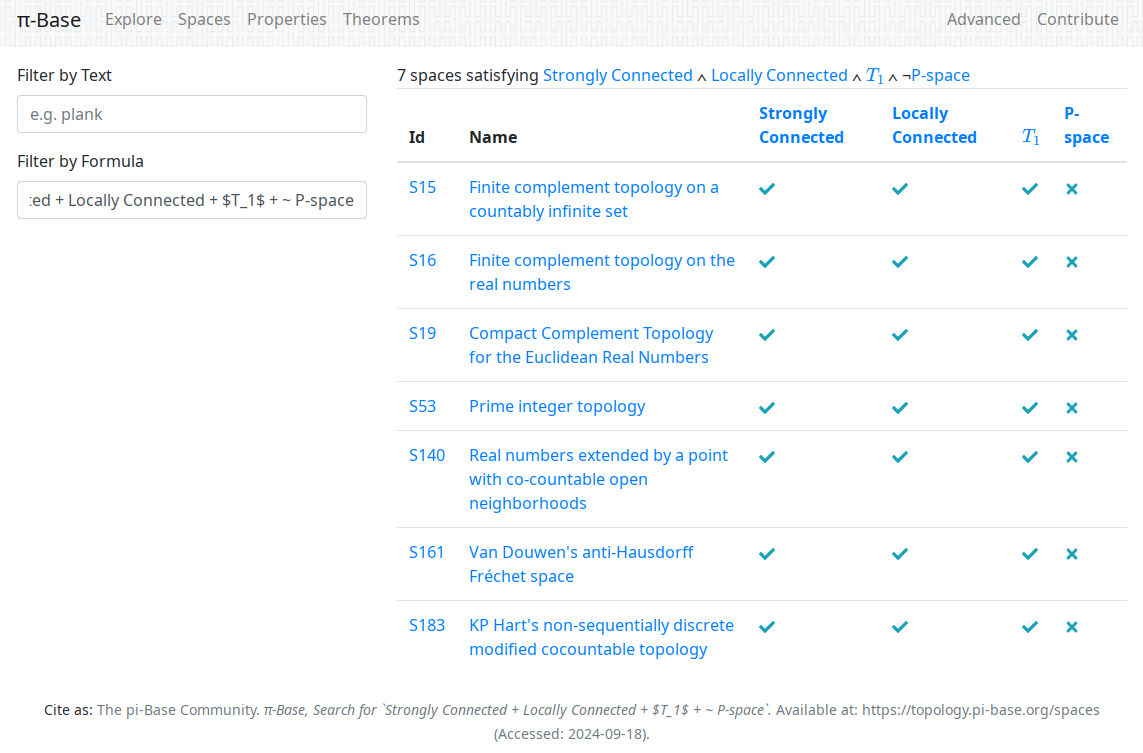
\includegraphics[width=\textwidth]{pi-base.png}
    \end{figure}

    \note{
        So we find the desired topos of sheaves over the cofinite topology on the naturals.

        But, we still need to manually verify it actually works, since the topological properies in the pi-base do not exactly mirror the interesting properties arising from topos theory.

        And in fact, there was a lot of fussing with translation before I could type something into the pi-base, even though I knew the exact properties I want. So wouldn't it be nice to have a similar site but whose objects are toposes? Actually, this inspired me to start working on this, so if anybody is interested please do ask me about it.
    }
\end{frame}

\end{document}
